\documentclass{article}
\usepackage[a4paper,bottom = 0.4in,left = 1in,right = 1in,top = 1in]{geometry}
\usepackage{graphicx} % Required for inserting images
\usepackage{verbatim}
\usepackage[utf8]{inputenc}
\usepackage{graphicx}
\usepackage{float}
\usepackage{fancyvrb}
\usepackage{varwidth}
\usepackage{amsmath}
\usepackage{siunitx}
\usepackage{chngcntr}
\usepackage{subfig}
\usepackage{alphalph}
\usepackage{enumerate}
\usepackage{pgffor}

\title{Wavelets \\EE678}
\author{Mohit\\20D070052 }
\date{September 2023}

\begin{document}


\maketitle
\begin{figure}[H]
\begin{center}

\includegraphics[scale = 0.2]{LOGO.jpeg}
\end{center}
\end{figure}
\section{Student Details}
\begin{tabular}{ l l  }
 Name: & Mohit \\ 
 Roll No: & 20D070052  \\  
 Group No: &7\\
 Group Member: & Vinayak Goyal (20D070088)
\end{tabular}

\newpage

\section{Question 1}
Using any suitable numerical analysis software, generate the continuous time Daubechies' scaling functions and wavelets corresponding to increasing analysis lowpass filter lengths: 4, 6, 8, 10, 12 and so on. Again, use any suitable numerical analysis software to obtain the Fourier Transform magnitude of the scaling functions and wavelets.

\subsection{Solution 1}
For the first question we have first generated the basic functions to get the convolution and the size of filter. After that we have constructed a general function to plot the Daubechies Wavelet for a general lowpass filter length. For this purpose we have used the by default available library in python and have used the filter bank index as 0 and 1 for scaling functions and wavelets respectively. The results obtained from the code is given below :

\subsection{Plots}

We have plotted the scaling functions and wavelets along with their fourier transform magnitude for lengths 2, 4, 6, .... upto 76 which can be seen in the code file including the plots for some of the lengths to show the trend.

\begin{figure}[H]
\begin{center}
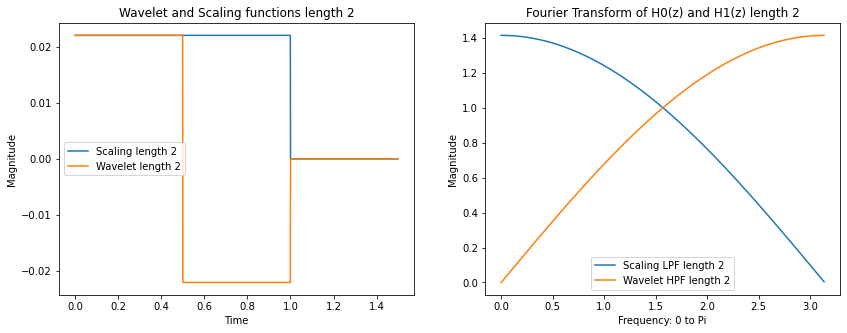
\includegraphics[scale = 0.5]{2.png}
\end{center}
\end{figure}

\begin{figure}[H]
\begin{center}
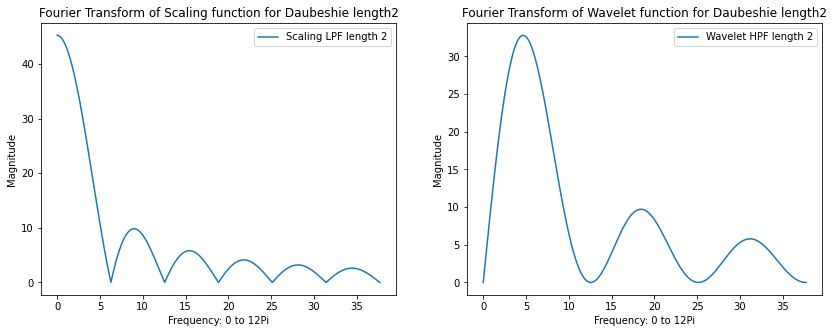
\includegraphics[scale = 0.5]{2f.png}
\end{center}
\end{figure}

\begin{figure}[H]
\begin{center}
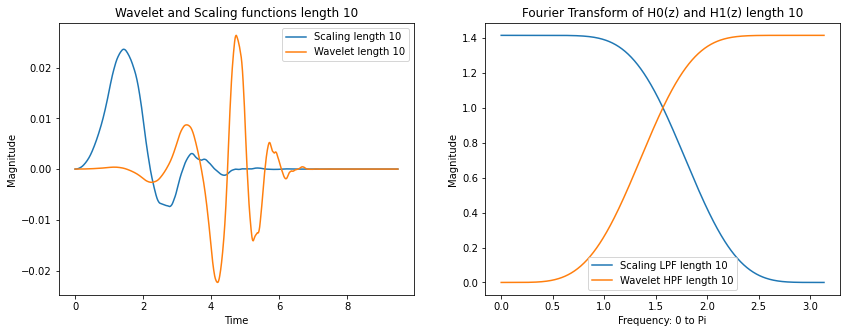
\includegraphics[scale = 0.5]{10.png}
\end{center}
\end{figure}

\begin{figure}[H]
\begin{center}
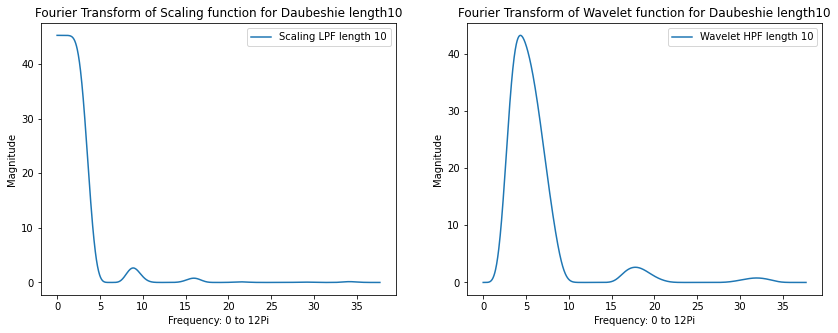
\includegraphics[scale = 0.5]{10f.png}
\end{center}
\end{figure}

\begin{figure}[H]
\begin{center}
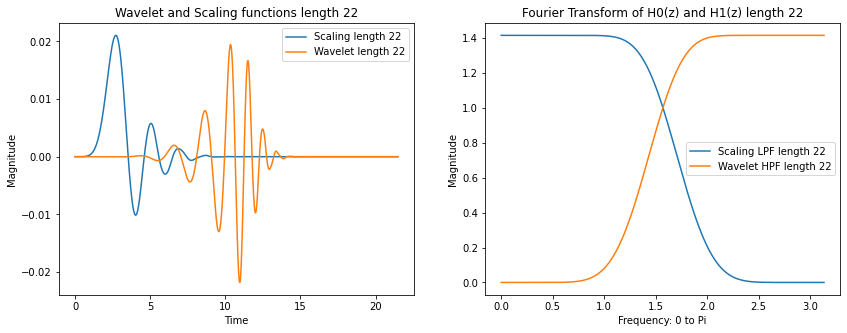
\includegraphics[scale = 0.5]{22.png}
\end{center}
\end{figure}

\begin{figure}[H]
\begin{center}
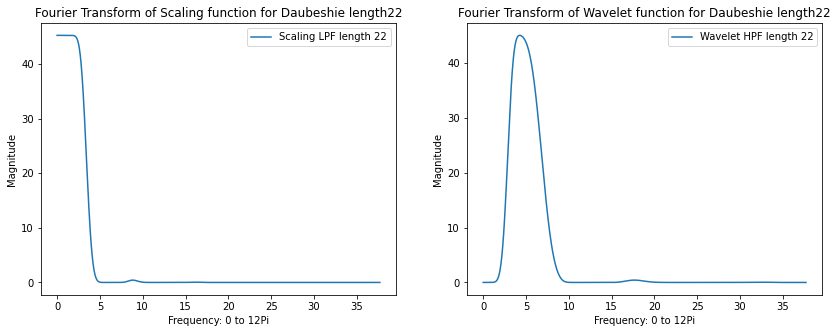
\includegraphics[scale = 0.5]{22f.png}
\end{center}
\end{figure}

\begin{figure}[H]
\begin{center}
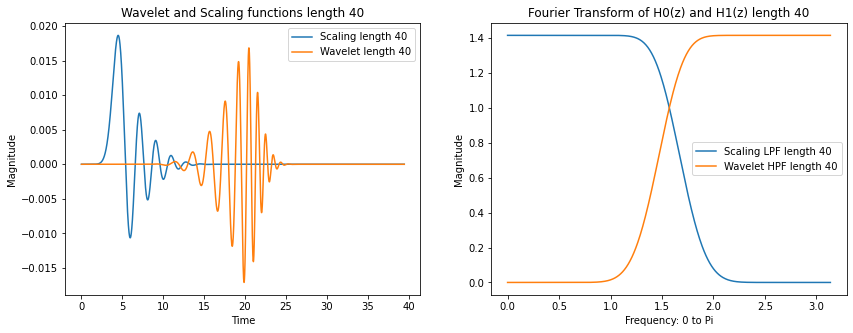
\includegraphics[scale = 0.5]{40.png}
\end{center}
\end{figure}

\begin{figure}[H]
\begin{center}
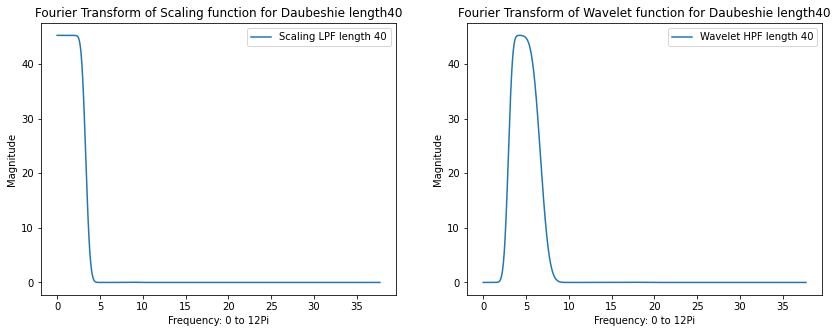
\includegraphics[scale = 0.5]{40f.png}
\end{center}
\end{figure}

\begin{figure}[H]
\begin{center}
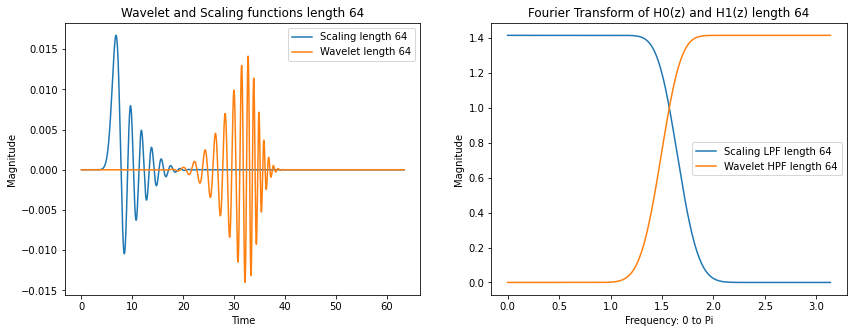
\includegraphics[scale = 0.5]{64.png}
\end{center}
\end{figure}

\begin{figure}[H]
\begin{center}
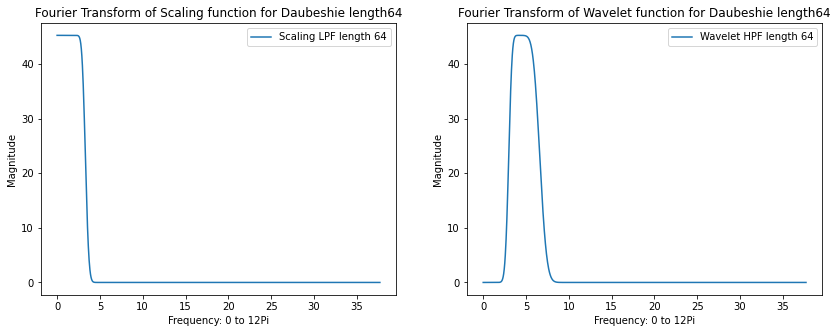
\includegraphics[scale = 0.5]{64f.png}
\end{center}
\end{figure}

\begin{figure}[H]
\begin{center}
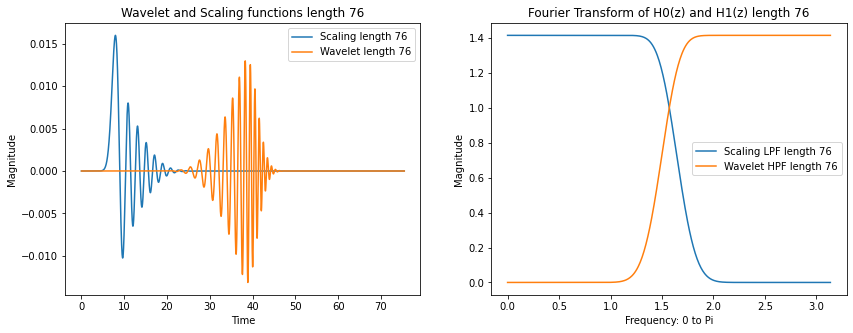
\includegraphics[scale = 0.5]{76.png}
\end{center}
\end{figure}

\begin{figure}[H]
\begin{center}
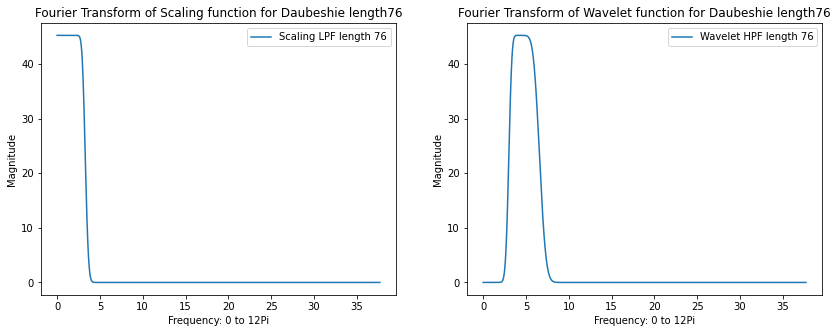
\includegraphics[scale = 0.5]{76f.png}
\end{center}
\end{figure}
\subsection{Observations}

If we observe the trend from the plots carefully we see that as we keep on increasing the length of Daubechies filter the plots tend to go towards an ideal low pass filter (LPF) and an ideal high pass filter (HPF) which is expected.

\section{Question 2}
Using any suitable numerical analysis software, obtain the time centre of each of the scaling functions and wavelets. What is the angular frequency centre of each of these functions? Thus, using any suitable numerical analysis software, obtain the time variance and the angular frequency variance of each of these scaling functions and wavelets. Tabulate, plot and study the trend of these variances and the product of these variances, with increasing filter length.

\subsection{Solution 2}

For this part we need to calculate the time centre, frequency centre, time variance and frequency variance with increasing length for analysis lowpass filters also we have showed this variation for increasing length of Daubechies filter. Therefore first we have defined the function to calculate the norm of x which will be the denominator for calculating time centre. After that we have defined the function to compute time centre. We also need to calculate the nth moments i.e. beyond centre and variance therefore we have defined a function for the same.

\subsection{Plots}

Here we have shown the plots for the variation of time centre on increasing the analysis lowpass filter length for scaling and wavelet functions for different lengths of Daubechies filter. Also we have shown the plot for product of time and frequency variance.

\begin{figure}[H]
\begin{center}
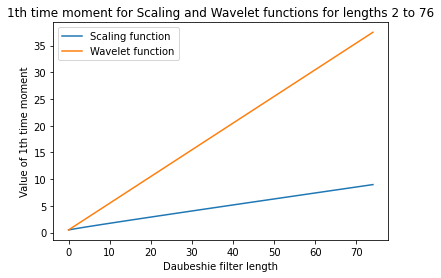
\includegraphics[scale = 0.8]{1th.png}
\end{center}
\end{figure}

\begin{figure}[H]
\begin{center}
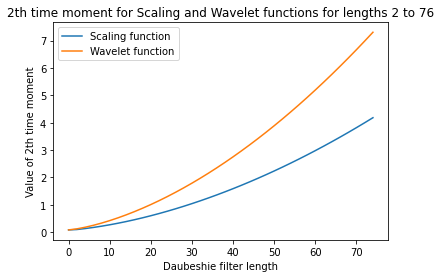
\includegraphics[scale = 0.8]{2nd.png}
\end{center}
\end{figure}

\begin{figure}[H]
\begin{center}
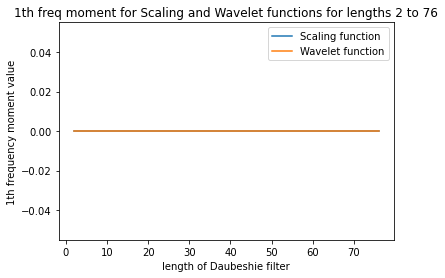
\includegraphics[scale = 0.8]{1th_f.png}
\end{center}
\end{figure}

\begin{figure}[H]
\begin{center}
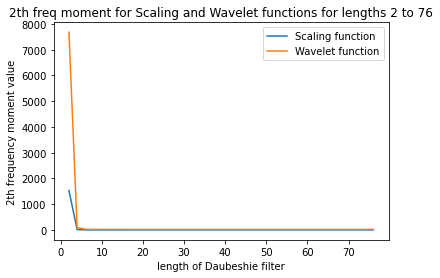
\includegraphics[scale = 0.8]{2nd_f.png}
\end{center}
\end{figure}

\begin{figure}[H]
\begin{center}
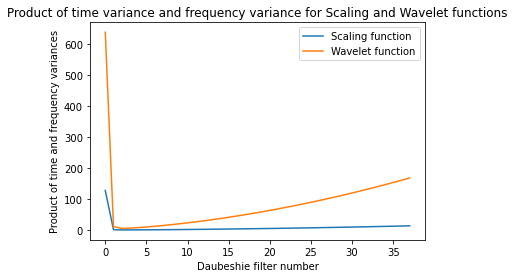
\includegraphics[scale = 0.8]{product2.png}
\end{center}
\end{figure}

\subsection{Observations}

\begin{itemize}

\item The time centre for both the scaling function as well as the wavelet function increases linearly with the analysis lowpass filter length however the slope for scaling function is larger than the wavelet function.

\item The time variance has the same trend that both the scaling function as well as the wavelet function increases however not linearly but exponentially with scaling function increasing faster than the wavelet function.

\item Here we can observe the plot of frequency centre that it is constantly zero for all lengths for both scaling functions and wavelets.

\item The frequency variance centre is very high for both the scaling and wavelet function at low length however both of them decreases abruptly as the length increases initially after which it is almost constant near zero for both of them. Also we can observe that the for scaling function the frequency variance is higher than the wavelet function.

\item The plot of product of time variance and frequency variance first decreases abruptly on increasing the length and thereafter it starts increasing for both the functions with scaling always higher than wavelet as expected. Also we can attribute the initial decrease due to the frequency variance and the increase thereafter to the time variance.

\end{itemize}


\section{Question 3}
Now, using any suitable numerical analysis software, estimate higher order moments of these scaling functions and wavelets, around the time centre in the time domain and around the angular frequency centre, in the Fourier domain. Do we see any trend? This is an open question, I do not believe the final word on this has been said. Explore if these higher order moments can be linked to the generalization of the Cauchy Schwartz inequality to other Lp spaces.

\subsection{Solution}

Here firstly we have defined a function to get the values of mth moment in time and frequency domain around time and frequency centre respectively for nth Daubechies Filter length. The results obtained from this analysis is as shown below, we will divide this problem into multiple subparts to observe each treand separately.

\subsection{Plots for mth time moments with increasing lowpass filter length}

\begin{figure}[H]
    \centering
    \subfloat[\centering]{{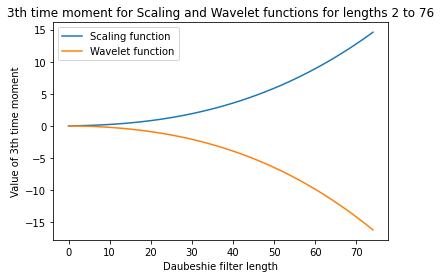
\includegraphics[width=7cm]{3rd.png} }}%
    \qquad
    \subfloat[\centering]{{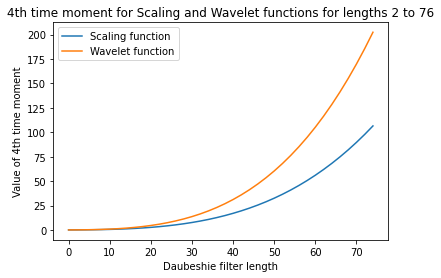
\includegraphics[width=7cm]{4th.png} }}%
    \label{fig:example}%
\end{figure}

\begin{figure}[H]
    \centering
    \subfloat[\centering]{{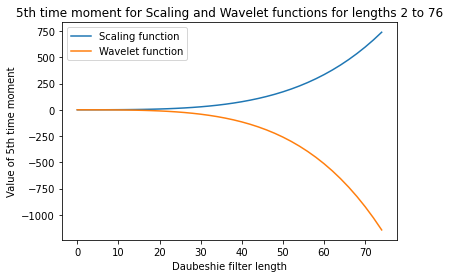
\includegraphics[width=7cm]{5th.png} }}%
    \qquad
    \subfloat[\centering]{{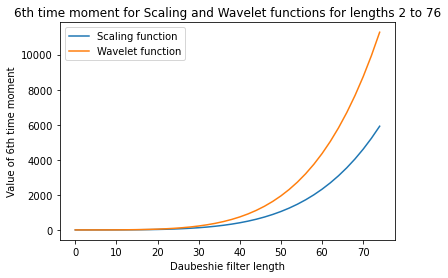
\includegraphics[width=7cm]{6th.png} }}%
    \label{fig:example}%
\end{figure}

\begin{figure}[H]
    \centering
    \subfloat[\centering]{{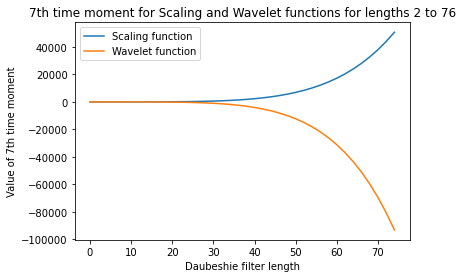
\includegraphics[width=7cm]{7th.png} }}%
    \qquad
    \subfloat[\centering]{{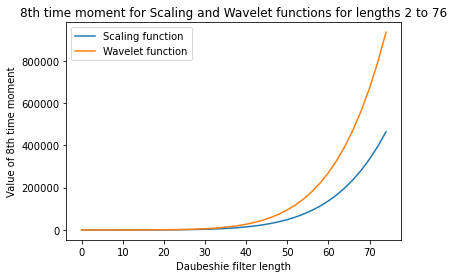
\includegraphics[width=7cm]{8th.png} }}%
    \label{fig:example}%
\end{figure}

\begin{figure}[H]
    \centering
    \subfloat[\centering]{{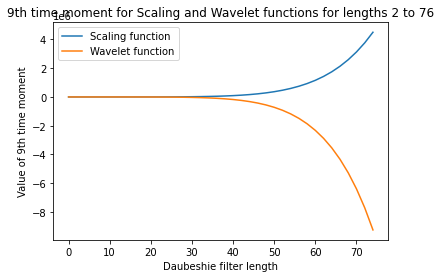
\includegraphics[width=7cm]{9th.png} }}%
    \qquad
    \subfloat[\centering]{{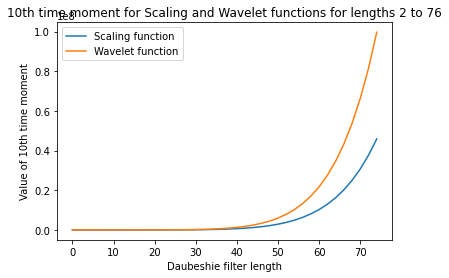
\includegraphics[width=7cm]{10th.png} }}%
    \label{fig:example}%
\end{figure}

\subsubsection{Observation}

\begin{itemize}
\item For larger time moments also the wavelet function keeps on increasing exponentially at a much faster rate.
\item The scaling function starts decreasing for odd time moments which are greater than 1 with faster rate than the wavelet function.
\item For even time moments scaling function increases faster than wavelet function and the values also increase as we increase the moment number.

\end{itemize}

\subsection{Plots for value of time moments for varying Daubechies Filter Length}

\begin{figure}[H]
    \centering
    \subfloat[\centering]{{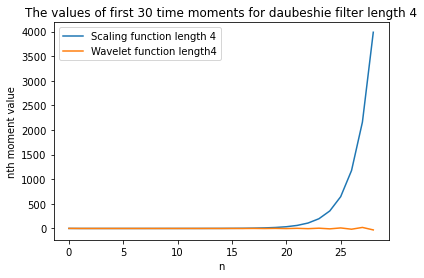
\includegraphics[width=7cm]{time4.png} }}%
    \qquad
    \subfloat[\centering]{{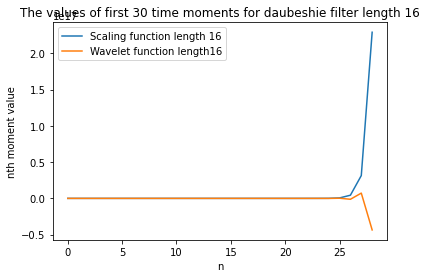
\includegraphics[width=7cm]{time16.png} }}%
    \label{fig:example}%
\end{figure}

\begin{figure}[H]
    \centering
    \subfloat[\centering]{{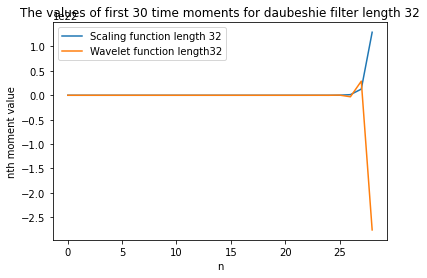
\includegraphics[width=7cm]{time32.png} }}%
    \qquad
    \subfloat[\centering]{{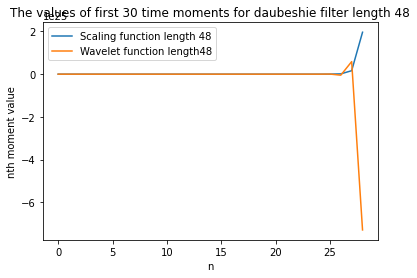
\includegraphics[width=7cm]{time48.png} }}%
    \label{fig:example}%
\end{figure}

\begin{figure}[H]
    \centering
    \subfloat[\centering]{{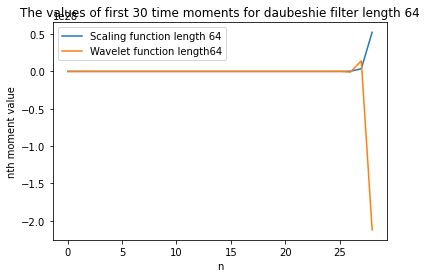
\includegraphics[width=7cm]{time64.png} }}%
    \qquad
    \subfloat[\centering]{{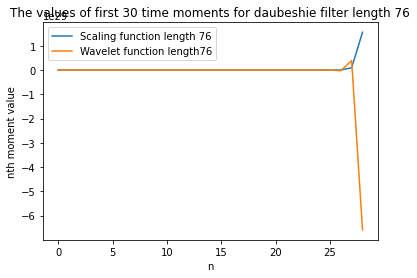
\includegraphics[width=7cm]{time76.png} }}%
    \label{fig:example}%
\end{figure}

\subsubsection{Observation}
\begin{itemize}
\item As we increase the filter length the value of time moments keep on increasing as we can see from the scale of graph on y axis.
\item These plots verify the trend that we observed from the previous plots that for odd moment scaling function is negative and for even moment the scaling function is higher than wavelet function.
\item For higher moments we also observe that the value for scaling function decreases very fast.
\end{itemize}

\subsection{Plots for mth frequency moments with increasing lowpass filter length}

\begin{figure}[H]
    \centering
    \subfloat[\centering]{{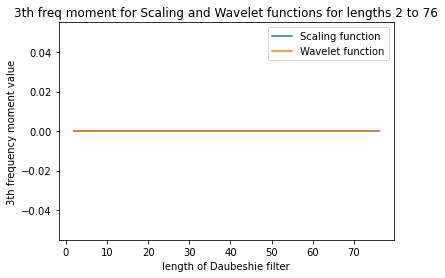
\includegraphics[width=7cm]{3rd_f.png} }}%
    \qquad
    \subfloat[\centering]{{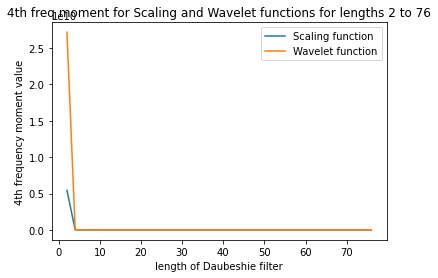
\includegraphics[width=7cm]{4th_f.png} }}%
    \label{fig:example}%
\end{figure}

\begin{figure}[H]
    \centering
    \subfloat{{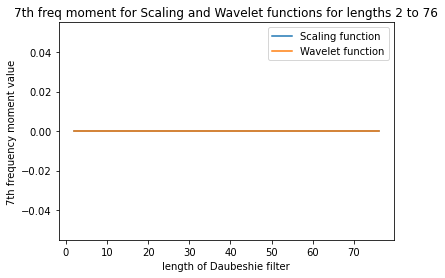
\includegraphics[width=7cm]{7th_f.png} }}%
    \qquad
    \subfloat{{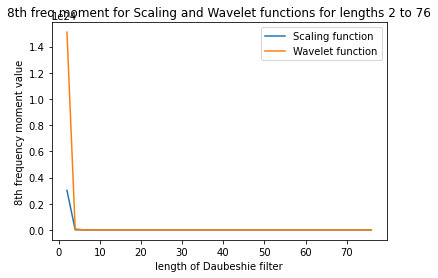
\includegraphics[width=7cm]{8th_f.png} }}%
    \label{fig:example}%
\end{figure}

\begin{figure}[H]
    \centering
    \subfloat[\centering]{{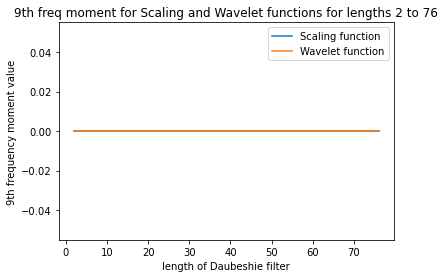
\includegraphics[width=7cm]{9th_f.png} }}%
    \qquad
    \subfloat[\centering]{{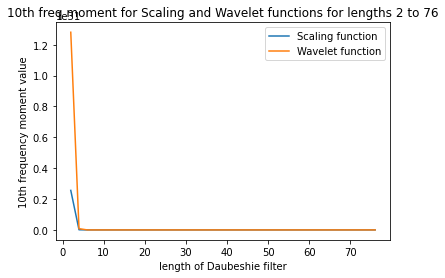
\includegraphics[width=7cm]{10th_f.png} }}%
    \label{fig:example}%
\end{figure}

\subsubsection{Observation}
\begin{itemize}
\item All the odd frequency moments are zero which is expected since the first frequency moment is zero.
\item For odd moments the trend is similar to the frequency variance trend but as we increase the moment number the starting point i.e. at low length increases.
\end{itemize}

\subsection{Plots for value of frequency moments for varying Daubechies Filter Length}

\begin{figure}[H]
    \centering
    \subfloat[\centering]{{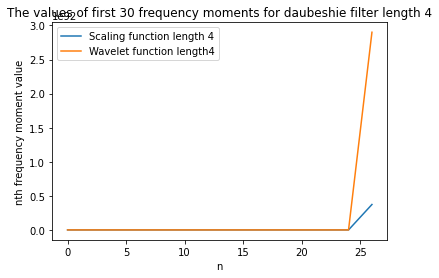
\includegraphics[width=7cm]{freq4.png} }}%
    \qquad
    \subfloat[\centering]{{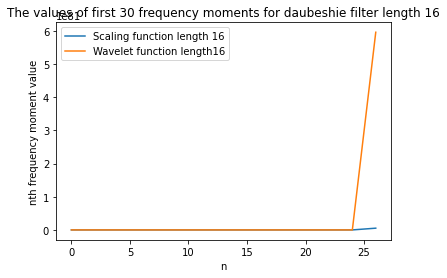
\includegraphics[width=7cm]{freq16.png} }}%
    \label{fig:example}%
\end{figure}

\begin{figure}[H]
    \centering
    \subfloat[\centering]{{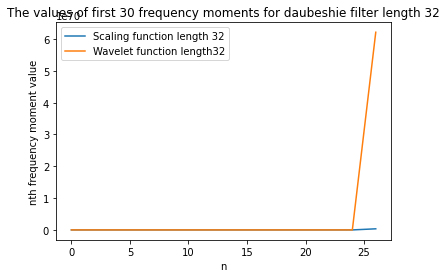
\includegraphics[width=7cm]{freq32.png} }}%
    \qquad
    \subfloat[\centering]{{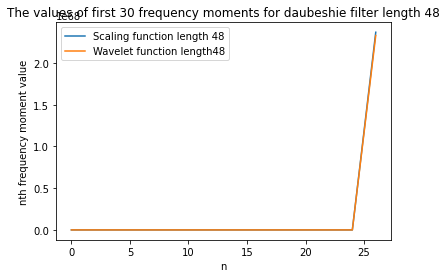
\includegraphics[width=7cm]{freq48.png} }}%
    \label{fig:example}%
\end{figure}

\begin{figure}[H]
    \centering
    \subfloat[\centering]{{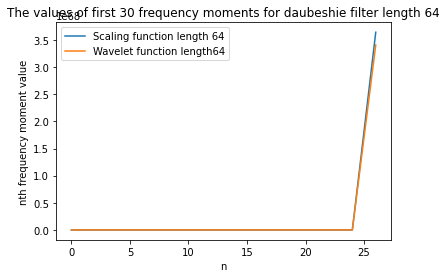
\includegraphics[width=7cm]{freq64.png} }}%
    \qquad
    \subfloat[\centering]{{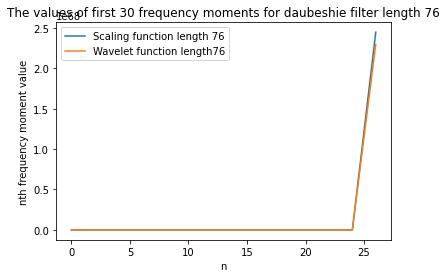
\includegraphics[width=7cm]{freq76.png} }}%
    \label{fig:example}%
\end{figure}

\subsubsection{Observation}
\begin{itemize}
\item The values of frequency moment increases with increasing the moment number.
\item With increasing length of filter the value of moments initially increases slowly upto some moment and then increases faster.
\end{itemize}

\subsection{Plots for product of time moments and frequency moments}

\begin{figure}[H]
\begin{center}
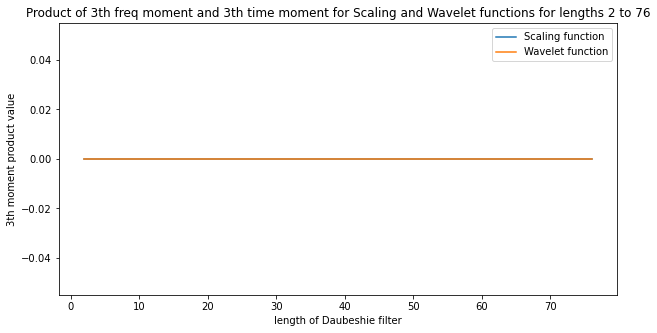
\includegraphics[scale = 0.6]{prod3.png}
\end{center}
\end{figure}

\begin{figure}[H]
\begin{center}
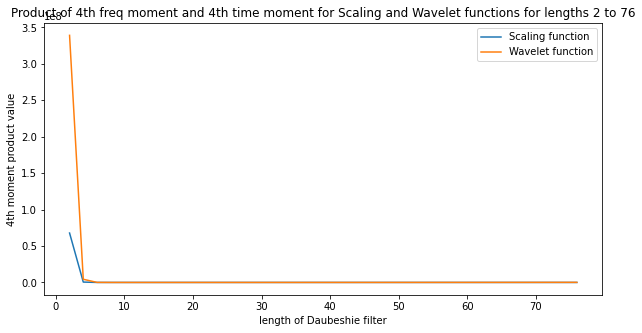
\includegraphics[scale = 0.6]{prod4.png}
\end{center}
\end{figure}

\begin{figure}[H]
\begin{center}
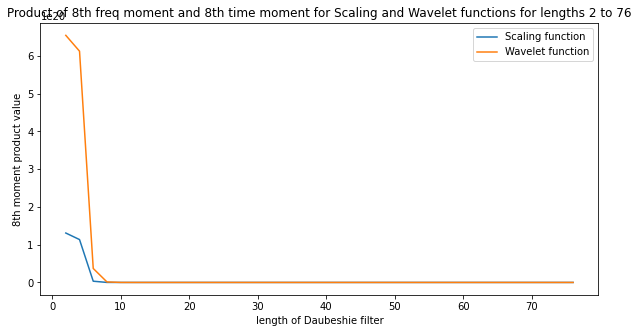
\includegraphics[scale = 0.6]{prod8.png}
\end{center}
\end{figure}

\begin{figure}[H]
\begin{center}
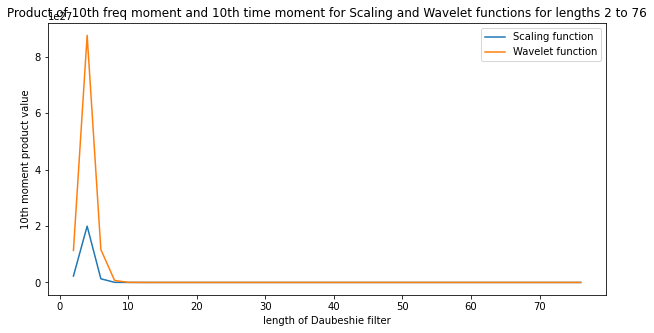
\includegraphics[scale = 0.6]{prod10.png}
\end{center}
\end{figure}

\subsubsection{Observation}
\begin{itemize}
\item All the odd products will be zero because the odd frequency moments are zero hence the product is zero.
\item The product increases with increase in the moment number used but abruptly decreases which is due to the trend that we saw in the frequency moments.

\end{itemize}


\section{Acknowledgement and Conclusion}
Therefore the midsem assignment is competed. Thanks a lot to Professor Gadre to give such a great learning assignment.



\end{document}